\section{Лема за покачването}

В този раздел ще разгледаме едно твърдение, което ще ни даде критерий за проверка кога един език не е безконтекстен. Ще започнем с няколко помощни твърдения.

\begin{proposition}\label{pr:pumping:ground}
  За произволни променливи $A$, $B$ и думи $\alpha_1,\alpha_2, \alpha_3$ е изпълнено:
  \begin{prooftree}
    \AxiomC{$A \yield{\ell_1}\alpha_1B\alpha_3$}
    \AxiomC{$B \yield{\ell_2} \alpha_2$}
    \BinaryInfC{$A \yield{ \leq \ell_1+\ell_2} \alpha_1\alpha_2\alpha_3$}
  \end{prooftree}
\end{proposition}
\begin{hint}
  Формално доказателството протича с индукция по $\ell_1$.
  
  \begin{figure}[H]
    \begin{subfigure}[t]{0.5\textwidth}
      \centering
      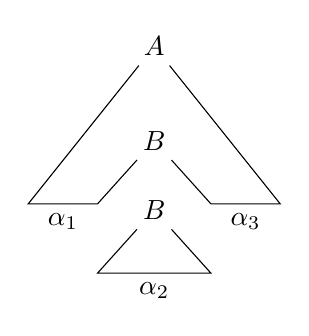
\begin{tikzpicture}[scale=0.8]
        \node (A) at (0,0) {$A$};
        \coordinate (B) at (-2,-2.5);
        \coordinate (C) at (2,-2.5);
        \coordinate (D) at (-0.9,-2.5);
        \coordinate (E) at (0.9,-2.5);
        \node (F) at (0,-1.5) {$B$};
        
        \node (G) at (0,-2.6) {$B$};
        \coordinate (H) at (-0.9,-3.6);
        \coordinate (I) at (0.9,-3.6);
        
        \draw (A) -- (B) -- node[below]{$\alpha_1$} (D) -- (F) -- (E) -- node[below]{$\alpha_3$} (C) -- (A);
        \draw (G) -- (H) -- node[below]{$\alpha_2$}(I) -- (G);
        
        % \draw [photon] (A) -- node[left]{$\alpha$} (F);
      \end{tikzpicture}
      \caption{\scriptsize{Синтактични дървета за изводите $A \yield{\ell_1}\alpha_1B\alpha_3$ и $B \yield{\ell_2} \alpha_2$}}
    \end{subfigure}
    % $\stackrel{\lambda}{\Rightarrow}$
    ~
    \begin{subfigure}[t]{0.5\textwidth}
      \centering
      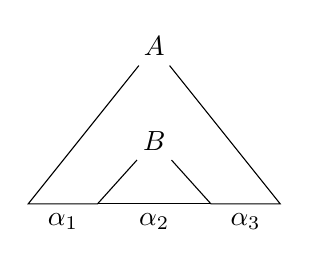
\begin{tikzpicture}[scale=0.8]
        \node (A) at (0,0) {$A$};
        \coordinate (B) at (-2,-2.5);
        \coordinate (C) at (2,-2.5);
        \coordinate (D) at (-0.9,-2.5);
        \coordinate (E) at (0.9,-2.5);
        \node (F) at (0,-1.5) {$B$};
        
        % \coordinate (G) at (0,-2.3) {${\scriptstyle X_\alpha}$};
        % \coordinate (H) at (-0.9,-3.3);
        % \coordinate (I) at (0.9,-3.3);
        
        \draw (A) -- (B) -- node[below]{$\alpha_1$} (D) -- (F) -- (E) -- node[below]{$\alpha_3$} (C) -- (A);
        \draw (D) -- node[below]{$\alpha_2$} (E);
      \end{tikzpicture}
      \caption{\scriptsize{Съединяваме двете дървета}}
      % \caption{$\texttt{yield}(\uppercut{P}{\alpha}) = \omega_1 \cdot \texttt{root}(\lowercut{P}{\alpha}) \cdot \omega_2$}
    \end{subfigure}
  \end{figure}
\end{hint}

\begin{proposition}\label{pr:pumping:iteration}
  За произволна променлива $A$ и произволни думи $\beta$ и $\gamma$ е изпълнено:
  \begin{prooftree}
    \AxiomC{$A \yield{\ell} \beta A \gamma$}
    \AxiomC{$i \in \Nat$}
    \BinaryInfC{$A \yield{\leq i \cdot \ell} \beta^i A \gamma^i$}
  \end{prooftree}
\end{proposition}
\begin{hint}
  Формално доказателството трябва да следва индукция по $i$.
  Понеже това доказателство не крие изненади, ще се задоволим с един пример. Нека $P$ да бъде синтактично дърво съответстващо на извода $A \yield{\ell} \beta A \gamma$.
  Тогава можем да получим синтактично дърво $P^{(2)}$  съответстващо на $A \yield{\leq 2\ell} \beta^2A\gamma^2$ по следния начин.
  \begin{figure}[H]
    \begin{subfigure}[t]{0.3\textwidth}
      \centering
      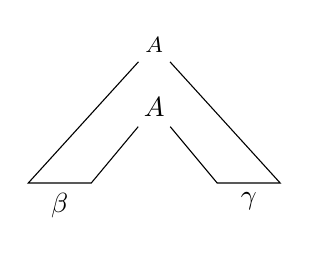
\begin{tikzpicture}[scale=0.8]
        \node (A) at (0,0) {\footnotesize{$A$}};
        \coordinate (B) at (-2,-2.2);
        \coordinate (C) at (2,-2.2);
        \coordinate (S) at (-1,-2.2);
        \coordinate (T) at (1,-2.2);
        \node (L) at (0,-1) {$A$};
        
        \draw (A) -- (B) -- node[below]{$\beta$}(S) -- (L) -- (T) -- node[below]{$\gamma$}(C) -- (A);
      \end{tikzpicture}
      \caption{\scriptsize{Синтактично дърво $P$ за извода $A \yield{\ell} \beta A\gamma$}}
    \end{subfigure}
    ~
    \begin{subfigure}[t]{0.3\textwidth}
      \centering
      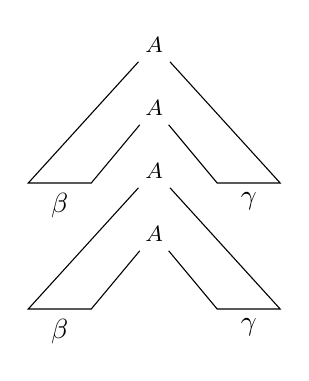
\begin{tikzpicture}[scale=0.8]
        \node       (A) at (0,0) {\footnotesize{$A$}};
        \coordinate (B) at (-2,-2.2);
        \coordinate (C) at (2,-2.2);
        \coordinate (S) at (-1,-2.2);
        \coordinate (T) at (1,-2.2);
        \node       (L) at (0,-1) {\footnotesize{$A$}};
        
        \coordinate (E) at (-0.7,-2.5);
        \coordinate (F) at (0.7,-2.5);
        
        
        \node       (H) at (0,-2) {\footnotesize{$A$}};
        \node       (X) at (0,-3) {\footnotesize{$A$}};
        \coordinate (D) at (-2,-4.2);
        \coordinate (G) at (2,-4.2);
        \coordinate (E) at (-1,-4.2);
        \coordinate (F) at (1,-4.2);
        
        \draw (A) -- (B) -- node[below]{$\beta$}(S) -- (L) -- (T) -- node[below]{$\gamma$}(C) -- (A);
        \draw (H) -- (D) -- node[below]{$\beta$}(E) -- (X) -- (F) -- node[below]{$\gamma$}(G) -- (H);
      \end{tikzpicture}
      \caption{\scriptsize{Съединяваме две копия на $P$}}
    \end{subfigure}
    ~
    \begin{subfigure}[t]{0.3\textwidth}
      \centering
      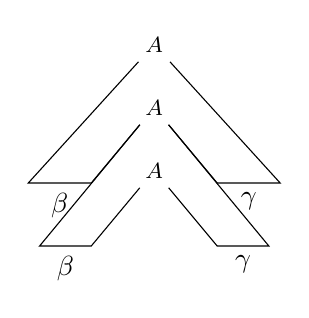
\begin{tikzpicture}[scale=0.8]
        \node       (A) at (0,0) {\footnotesize{$A$}};
        \coordinate (B) at (-2,-2.2);
        \coordinate (C) at (2,-2.2);
        \coordinate (S) at (-1,-2.2);
        \coordinate (T) at (1,-2.2);
        \node       (L) at (0,-1) {\footnotesize{$A$}};
        
        \coordinate (E) at (-0.7,-2.2);
        \coordinate (F) at (0.7,-2.2);
        
        \node       (X) at (0,-2) {\footnotesize{$A$}};
        \coordinate (D) at (-1.82,-3.2);
        \coordinate (G) at (1.82,-3.2);
        \coordinate (E) at (-1,-3.2);
        \coordinate (F) at (1,-3.2);
        
        \draw (A) -- (B) -- node[below]{$\beta$}(S) -- (L) -- (T) -- node[below]{$\gamma$}(C) -- (A);
        \draw (L) -- (D) -- node[below]{$\beta$}(E) -- (X) -- (F) -- node[below]{$\gamma$}(G) -- (L);
      \end{tikzpicture}
      \caption{\scriptsize{Получаваме синтактично дърво $P^{(2)}$ за извода $A \yield{\leq 2\ell} \beta^2 A \gamma^2$}}
    \end{subfigure}
  \end{figure}
\end{hint}

\begin{proposition}\label{pr:pumping:lower-bound}
  Нека $G$ е безконтекстна граматика и 
  \[b \df \max\{\ |\gamma| \mid A \to \gamma \text{ е правило в }G\ \}.\]
  Тогава:
  \begin{itemize}
  \item 
    Ако $A \yield{\leq\ell} \alpha$, то $|\alpha| \leq b^\ell$.
  \item
    Ако $\alpha \in \L(G)$ и $|\alpha| > b^\ell$, то $S \yield{\geq \ell+1} \alpha$.
  \end{itemize}
\end{proposition}
\begin{proof}

%   \begin{proposition}
%   \label{cor:tree:upper-bound}
%   \mynote{Това следствие ще бъде важно за нас, когато разгледаме лемата за покачването за безконтекстни езици.}
%   Нека $P = (T,\lambda)$ е дърво на извод съвместимо с $G$. Тогава
%   \[|\texttt{yield}(P)| \leq b^{{\high}(P)}.\]
% \end{proposition}
% \begin{proof}
%   Следва директно от горното твърдение след като съобразим, че
%   \[|\texttt{yield}(P)| \leq |\leaves(P)|.\]
% \end{proof}

  
  Това твърдение е на практика следствие от \Problem{tree:leaves-upper-bound} в комбинация с \Proposition{yield-relation:parse-tree}.
  \begin{itemize}
  \item
    Да разгледаме синтактично дърво $P = (T,\lambda)$ за извода $A \yield{\leq\ell} \alpha$.
    Според \Problem{tree:leaves-upper-bound} имаме, че $\abs{\alpha} = \abs{\leaves(T)}\leq b^{\high(T)} = b^{\ell}$.
  \item
    Нека $\alpha \in \L(G)$. Това означава, че $S \yield{\star} \alpha$.
    Ако допуснем, че $S \yield{\leq \ell} \alpha$, то бихме имали, че $\abs{\alpha} \leq b^\ell$, което е противоречие.
    Заключаваме, че $S \yield{\geq \ell+1} \alpha$.
  \end{itemize}
\end{proof}

\begin{important}
  \begin{lemma}[за покачването (безконтекстни езици)]
    \index{лема за покачването!безконтекстни езици}
    \label{lem:pumping-context} 
    \mynote{\cite[стр. 125]{sipser3}, \cite[стр. 125]{hopcroft1}, \cite[стр. 148]{kozen}}
    За всеки безконтекстен език $L$ съществува $p>0$, такова
    че ако $\alpha\in L$, за която $\abs{\alpha} \geq p$, то съществува разбиване на думата на пет части, $\alpha=xyuvw$,
    \mynote{Ще казваме, че $p$ е константа на покачването. Тук отново да напомним, че $0 \in \Nat$ и $xy^0uv^0w = xuw$.}
    за което е изпълнено:
    \begin{enumerate}[1)]
    \item
      $\abs{yv}\geq 1$,
    \item
      $\abs{yuv}\leq p$, и
    \item
      $(\forall i\in\Nat)[xy^iuv^iw\in L]$.
    \end{enumerate}
  \end{lemma}
\end{important}
\begin{proof}
  \mynote{Числото $b$ е максималната разклоненост на всяко дърво на извод за дума изводима от граматиката $G$.}
  Нека $G$ е безконтекстна граматика за езика $L$. Да положим
  \[p \df b^{\abs{V}+1}, \text{ където }b \df \max\{\ |\gamma| \mid A \to \gamma \text{ е правило в }G\ \}.\]
  Ще покажем, че този избор на $p$ е удачен за удовлетворяването на условията на лемата. Ще наричаме $p$ константа на покачването за граматиката $G$.
  
  Да разгледаме произволна дума $\alpha \in \L(G)$, за която $\abs{\alpha} \geq p$.
  Понеже $\L(G)$ е безкраен език, то със сигурност можем да намерим такава дума.
  Според \Proposition{pumping:lower-bound}, имаме $S \yield{\ell}\alpha$, където $\ell \geq \abs{V}+1$.
  Нека измежду всички синтактични дървета $P = (T,\lambda)$ за извода $S \yield{\star} \alpha$ сме избрали такова с \emph{минимален} брой върхове в дървото $T$.
  Да фиксираме \emph{максимален} път $\pi$ в $T$, т.е. дума $\pi \in T$ и $|\pi| = \ell$. Щом $\ell \geq \abs{V}+1$, то това означава, че по този път $\pi$
  се срещат поне $\abs{V}+1$ на брои променливи. От принципа на Дирихле следва, че трябва да има повторения на променливи по този път. 
  В $P$ можем да изберем това срещане на двойка повтарящи се променливи по пътя $\pi$, както на \Figure{pumping:partition}, което е възможно най-близо до края на пътя.
  Това означава, че можем да разбием извода $S \yield{\star} \alpha$ като $S \yield{\star} xAw$ и $A \yield{\leq \abs{V}+1} \gamma$, където $\alpha = x\gamma w$.
  Сега според нашия избор, изводът $A \yield{\leq \abs{V}+1} \gamma$ може да се разбие като $A \yield{\leq \abs{V}+1} yAv$ и $A \yield{\leq \abs{V}} u$,
  където $\gamma = yuv$.
  Да обобщим. Можем да разбием думата $\alpha$ на пет части като $\alpha = xyuvw$ с изводите:
  \begin{enumerate}[(1)]
  \item
    $S \yield{\star} x A w$, 
  \item
    $A \yield{\leq \abs{V}+1} y A v$, защото в $P$ можем да изберем това срещане на повтаряща се променлива по пътя $\pi$, което е възможно най-близо до листото.
  \item
    $A \yield{\leq \abs{V}} u$, като тук вече няма повтарящи се променливи по останалата част от пътя $\pi$.
  \end{enumerate}

  \begin{figure}[H]
    \begin{subfigure}[t]{0.3\textwidth}
    \centering
    \begin{tikzpicture}[scale=0.8]
      \node (A) at (0,0) {\footnotesize{$S$}};
      \coordinate (B) at (-2,-3);
      \coordinate (C) at (2,-3);
      \node (D) at (0,-1.2) {\footnotesize{$A$}};
      \coordinate (D1) at (1.4,-3);
      \coordinate (D2) at (-1.4,-3);
      \node (E) at (0,-2.3) {\footnotesize{$A$}};
      \coordinate (E1) at (0.7,-3);
      \coordinate (E2) at (-0.7,-3);
      \coordinate (F) at (0,-3);

      \draw (A) -- node[above left]{$P = $} (B) -- node[below]{$\pi$}(C) -- (A);
      \draw [photon2] (A) -- (D) -- (E) -- (F);
    \end{tikzpicture}
    \caption{Най-долните две повторения на променлива по пътя $\pi$.}
    \label{fig:pumping:partition}
  \end{subfigure}
  ~
  \begin{subfigure}[t]{0.3\textwidth}
    \centering
    \begin{tikzpicture}[scale=0.8]
      \node (A) at (0,0) {\footnotesize{$S$}};
      \coordinate (B) at (-2,-3);
      \coordinate (C) at (2,-3);
      \node (D) at (0,-1.2) {\footnotesize{$A$}};
      \coordinate (D1) at (1.4,-3);
      \coordinate (D2) at (-1.4,-3);
      \node (E) at (0,-2.3) {\footnotesize{$A$}};
      \coordinate (E1) at (0.5,-3);
      \coordinate (E2) at (-0.5,-3);
      \coordinate (F) at (0,-3);

      \draw (A) -- node[above left]{$P = $} (B) -- node[below] {$x$} (D2) -- (D) -- (D1) -- node[below]{$w$} (C) -- (A);
      \draw (D2) -- node[below]{$y$} (E2) -- (E) -- (E1) -- node[below]{$v$} (D1);
      \draw (E2) -- node[below]{$u$} (E1);

      \draw [photon2] (A) -- (D) -- (E) -- (F);
    \end{tikzpicture}
    \caption{Разбиваме дървото на три части.}
    \end{subfigure}
    ~
    \begin{subfigure}[t]{0.3\textwidth}
      \centering
      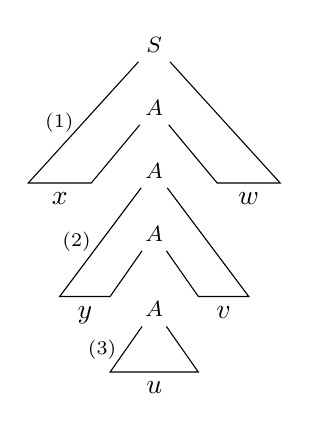
\begin{tikzpicture}[scale=0.8]
        \node (A) at (0,0) {\footnotesize{$S$}};
        \coordinate (B) at (-2,-2.2);
        \coordinate (C) at (2,-2.2);
        \coordinate (S) at (-1,-2.2);
        \coordinate (T) at (1,-2.2);
        \node (L) at (0,-1) {\footnotesize{$A$}};
        
        \coordinate (E) at (-0.7,-2.5);
        \coordinate (F) at (0.7,-2.5);
        
        
        \node (H) at (0,-2) {\footnotesize{$A$}};
        \node (X) at (0,-3) {\footnotesize{$A$}};
        \coordinate (D) at (-1.5,-4);
        \coordinate (G) at (1.5,-4);
        \coordinate (E) at (-0.7,-4);
        \coordinate (F) at (0.7,-4);
        
        \node (I) at (0,-4.2) {\footnotesize{$A$}};
        \coordinate (U) at (-0.7,-5.2);
        \coordinate (V) at (0.7,-5.2);
        
        \draw (A) -- node[left]{\scriptsize{(1)}}(B) -- node[below]{$x$}(S) -- (L) -- (T) -- node[below]{$w$}(C) -- (A);
        \draw (H) -- node[left]{\scriptsize{(2)}}(D) -- node[below]{$y$}(E) -- (X) -- (F) -- node[below]{$v$}(G) -- (H);
        \draw (I) -- node[left]{\scriptsize{(3)}}(U) -- node[below]{$u$}(V) -- (I);
      \end{tikzpicture}
      \caption{Получаваме три отделни синтактични дървета.}
    \end{subfigure}
  \end{figure}
  Сега остава да проверим условието на лемата:
  \begin{itemize}
  \item
    Да допуснем, че $\abs{yv} = 0$. Това означава, че $\alpha = xuw$ и имаме извода:
    \begin{prooftree}
      \AxiomC{$S \yield{\star} xAu$}
      \AxiomC{$A \yield{\star} u$}
      \RightLabel{\scriptsize{(\Proposition{pumping:ground})}}
      \BinaryInfC{$S \yield{\star} \underbrace{xuv}_{\alpha}$,}
    \end{prooftree}
    за който съществува дърво на извод с по-малко на брой възли отколкото $P$, защото махаме средната част, която съдържа поне един възел.
    Това е противоречие с избора на $P$ като синтактично дърво за $S \yield{\star}\alpha$ с минимален брой възли.
    Заключаваме, че $\abs{yv} \geq 1$.
  \item
    Понеже имаме извода $A \yield{\leq\abs{V}+1} yuv$, то от \Proposition{pumping:lower-bound} следва, че $\abs{yuv} \leq b^{\abs{V}+1} = p$.
  \item
    За произволно $i\in\Nat$ имаме извода:
    \begin{prooftree}
      \AxiomC{$A \yield{\star}yAv$}
      \LeftLabel{\scriptsize{(\Proposition{pumping:iteration})}}
      \UnaryInfC{$A \yield{\star}y^iAv^i$}
      \AxiomC{$A \yield{\star} u$}
      \LeftLabel{\scriptsize{(\Proposition{pumping:ground})}}
      \BinaryInfC{$A \yield{\star} y^iuv^i$}
      \AxiomC{$S \yield{\star}xAw$}
      \LeftLabel{\scriptsize{(\Proposition{pumping:ground})}}
      \BinaryInfC{$S \yield{\star} xy^iuv^iw$}
    \end{prooftree}
    Оттук заключаваме, че $(\forall i \in \Nat)[xy^iuv^iw \in \L(G)]$.
  \end{itemize}
\end{proof}

Както и при \Lemma{pumping-reg}, ние ще използваме \emph{контрапозицията} на условието на \Lemma{pumping-context}
при проверка, че даден език не е безконтекстен.

\begin{corollary}
  \label{cor:pumping-context-free}
  \mynote{Ако $L$ е краен език, то е ясно, че $L$ е безконтекстен.}
  Нека $L$ е произволен {\bf безкраен} език. Нека също така е изпълнено, че:
  \begin{description}
  \item[($\forall$)]
    за {\em всяко} естествено число $p \geq 1$,
  \item[($\exists$)]
    можем да намерим дума $\alpha \in L$, $\abs{\alpha}\geq p$, такава че
  \item[($\forall$)]
    за {\em всяко} разбиване на думата на пет части, $\alpha = xyuvw$, със свойствата $\abs{yv} \geq 1$ и $\abs{yuv} \leq p$,
  \item[($\exists$)]
    можем да намерим $i \in \Nat$, за което е изпълнено, че $xy^iuv^iw \not\in L$.
  \end{description}  
  \mynote{\writedown Докажете! Аналогично е на \Corollary{pumping-reg}}
  Тогава $L$ {\bf не} е безконтекстен език.
\end{corollary}

\begin{corollary}
  \mynote{\writedown Докажете!}
  Нека $G$ е безконтекстна граматика и $p$ е константата на покачването за $G$.
  Тогава $\abs{\L(G)} = \infty$ точно тогава, когато съществува $\alpha \in \L(G)$, за която $p \leq \abs{\alpha} < 2p$.
\end{corollary}
% \begin{proof}
%   Ако съществува дума $\alpha \in L$, за която $\abs{\alpha} \geq p$, то от \Lem{pumping-context} следва,
%   че $\abs{L} = \infty$, защото $\alpha = xyuvw$ и $xy^iuv^iw \in L$, за всяко $i\in\Nat$.

%   За другата посока, нека сега $\abs{L} = \infty$.
%   Да изберем най-късата дума $\alpha \in L$, за която $\abs{\alpha} \geq p$.
%   Ще докажем, че $p \leq \abs{\alpha} < 2p$. За целта да допуснем, че $\abs{\alpha} \geq 2p$.
%   Тогава от \Lem{pumping-context} следва, че $\alpha = xyuvw$, $\abs{yv} \geq 1$, $\abs{yuv} \leq p$, $xy^0uv^0w = xuw \in L$.
%   Ако $\abs{xuw} < p$, то $\abs{yv} > p$, защото $\abs{yv} + \abs{xuw} = \abs{\alpha} \geq 2p$, и следователно $\abs{yuv} > p$, което е противоречие.
%   Следва, че $\abs{\alpha} > \abs{xuw} \geq p$.
%   Получихме, че думата $xuw\in L$ и $\abs{xuw} \geq p$. Това е противоречие с минималността на $\alpha$.
% \end{proof}

% \begin{framed}
%   \Lem{pumping-context} е полезна, когато искаме да докажем, че даден език $L$ {\bf не} е безконтекстен.
%   За целта, доказваме отрицанието на свойствата от \Lem{pumping-context} за $L$, т.е.
%   за всяка константа $p$, ние намираме дума $\alpha \in L$, $\abs{\alpha}\geq p$, такава че за всяко разбиване на думата на пет части, $\alpha = xyuvw$,
%   със свойствата $\abs{yv} \geq 1$ и $\abs{yuv} \leq p$, е изпълнено, че $(\exists i)[xy^iuv^iw \not\in L]$.
% \end{framed}

\begin{remark}
  Алгоритъм за проверка дали един безконтекстен език е безкраен следвайки горния критерий би 
  имал експоненциална сложност относно $|G|$.
\end{remark}

\begin{example}
  \label{ex:anbncn}
  Да видим защо езикът $L = \{a^nb^nc^n\ \mid\ n\in\Nat\}$ не е безконтекстен.
  \begin{description}
  \item[$(\forall)$]
    Разглеждаме произволна константа $p \geq 1$.
  \item[$(\exists)$]
    Избираме дума $\alpha \in L$, $\abs{\alpha} \geq p$.
    В случая, нека $\alpha = a^pb^pc^p$.
  \item[$(\forall)$]
    Разглеждаме произволно разбиване $xyuvw = \alpha$, за което $\abs{yuv} \leq p$ и $1 \leq \abs{yv}$.
  \item[$(\exists)$]
    Ще изберем $i$, за което $xy^iuv^iw \not\in L$.
    Знаем, че поне едно от $y$ и $v$ не е празната дума.
    Имаме няколко случая за $y$ и $v$.
    \begin{itemize}
    \item
      $y$ и $v$ са думи съставени от една буква.
      В този случай получаваме, че $xy^2uv^2w$ има различен брой букви $a$, $b$ и $c$.
    \item
      $y$ или $v$ е съставена от две букви.
      Тогава е възможно да се окаже, че $xy^2uv^2w$ да има равен брой $a$, $b$ и $c$,
      но тогава редът на буквите е нарушен.
    \item
      понеже $\abs{yuv} \leq p$, то не е възможно в $y$ или $v$ да се срещат и трите букви.
    \end{itemize}  
    Оказа се, че във всички възможни случаи за $y$ и $v$, 
    $xy^2uv^2w \not\in L$.
  \end{description}
  Така от \Corollary{pumping-context-free} следва, че езикът $L$ не е безконтекстен.
\end{example}

\begin{framed}
  \begin{proposition}
    Безконтекстните езици {\bf не} са затворени относно сечение и допълнение.
  \end{proposition}
\end{framed}
\begin{hint}
  Да разгледаме езика $L_0 = \{a^nb^nc^n\mid n\in\Nat\}$, за който вече знаем от \Example{anbncn}, че не е безконтекстен.
  Да вземем също така и безконтекстните езици 
  \mynote{\writedown Защо $L_1$ и $L_2$ са безконтекстни?}
  \[L_1 = \{a^nb^nc^m\mid n,m\in\Nat\},\ L_2 = \{a^mb^nc^n\mid n,m\in\Nat\},\]
  \mynote{Озн. $\ov{L} \df \Sigma^\star \setminus L$}
  \begin{itemize}
  \item 
    Понеже $L_0 = L_1\cap L_2$, то заключаваме, че безконтекстните езици не са затворени 
    относно операцията сечение.
  \item
    \mynote{Друг пример, с който може да се види, че безконтекстните езици не са затворени относно допълнение е 
      като се докаже, че езикът
      \[\{a,b\}^\star \setminus \{\alpha\alpha\mid \alpha\in \{a,b\}^\star\}\]
      е безконтекстен.
      Това следва лесно като се използва \Problem{equal-but-different}.}
    Да допуснем, че безконтекстните езици са затворени относно операцията допълнение.
    Тогава  $\ov{L}_1$ и $\ov{L}_2$ са безконтекстни.
    Знаем, че безконтекстните езици са затворени относно обединение. 
    Следователно, езикът $L_3 = \ov{L}_1 \cup \ov{L}_2$ също е безконтекстен.
    Понеже допуснахме, че безконтекстните са затворени относно допълнение, то $\ov{L}_3$ също е безконтекстен.
    Но тогава получаваме, че езикът
    \[L_0 = L_1 \cap L_2 = \ov{\ov{L}_1 \cup \ov{L}_2} = \ov{L}_3\]
    е безконтекстен, което е противоречие.
  \end{itemize}
\end{hint}

%%% Local Variables:
%%% mode: latex
%%% TeX-master: "../eai"
%%% End:
